\section{Surfaces and nondegenerate symmetric bilinear forms}

We are aiming towards a proof of a fundamental cohomological property of
manifolds. 

\begin{definition} A (topological) manifold is a Hausdorff space such that
every point has an open neighborhood that is homeomorphic to some (finite
dimensional) Euclidean space. 
\end{definition}

If all these Euclidean spaces can be chosen to be $\RR^n$, we have an 
$n$-manifold. 

In this lecture we will state a case of the Poincar\'e duality theorem
and study some consequences of it, especially for compact 2-manifolds. 
This whole lecture will be happening with coefficients in $\FF_2$. 

\begin{theorem}
Let $M$ be a compact manifold of dimension $n$.  
There exists a unique class $[M]\in H_n(M)$, called the {\em fundamental class}, such that for every $p,q$ with $p+q=n$ the pairing 
\[
H^p(M)\otimes H^q(M)\xrightarrow{\cup} H^n(M)\xrightarrow{\langle -,[M]\rangle}\FF_2
\]
is perfect. 
\end{theorem}
This means that the adjoint map
\[
H^p(M)\to\Hom(H^q(M),\FF_2)
\]
is an isomorphism. Since cohomology vanishes in negative dimensions, one thing
this implies is that $H^p(M)=0$ for $p>n$. Since $M$ is compact, $\pi_0(M)$
is finite, and 
\[
H^n(M)=\Hom(H^0(M),\FF_2)=\Hom(\Map(\pi_0(M),\FF_2),\FF_2)=\FF_2[\pi_0(M)]\,.
\]
A vector space $V$ admitting a perfect pairing $V\otimes W\to\FF_2$
is necessarily finite dimensional; so $H^p(M)$ is in fact finite-dimensional 
for all $p$.

Combining this pairing with the universal coefficient theorem, we get 
isomorphisms
\[
H^p(M)\xrightarrow{\cong}\Hom(H^p(M),\FF_2)\xleftarrow{\cong}H_q(M)\,.
\]
The homology and cohomology classes corresponding to each other under this 
isomorphism are said to be ``Poincar\'e dual.'' 

Using these isomorphisms, the cup product pairing can be rewritten as a
homology pairing:
\[
\xymatrix{
H_p(M)\otimes H_q(M) \ar[r]^\pitchfork \ar[d]^\cong & 
H_{n-p-q}(M) \ar[d]^\cong \\
H^{n-p}(M)\otimes H^{n-q}(M) \ar[r]^\cup & H^{2n-p-q}(M)\,.
}\]
This is the {\em intersection pairing}. Here's how to think of it. 
Take homology classes $\alpha\in H_p(M)$ and $\beta\in H_q(M)$ and
represent them (if possible!) as the image of the fundamental classes
of submanifolds of $M$, of dimensions $p$ and $q$. 
Move them if necessary to make them intersect ``transversely.''
Then their intersection will be a submanifold of dimension
$n-p-q$, and it will represent the homology class $\alpha\pitchfork\beta$.

This relationship between the cup product and the intersection pairing is 
the source of the symbol for the cup product.

\begin{example}
Let $M=T^2=S^1\times S^1$. We know that 
\[
H^1(M)=\FF_2\langle a,b\rangle
\]
and $a^2=b^2=0$, while $ab=ba$ generates $H^2(M)$.
The Poincar\'e duals of these classes are represented by cycles $\alpha$
and $\beta$ wrapping 
around one or the other of the two factor circles. They can be made to 
intersect in a single point. This reflects the fact that 
\[
\langle a\cup b,[M]\rangle=1\,.
\]
Similarly, the fact that $a^2=0$ reflects the fact that its Poincar\'e 
dual cycle $\alpha$ can be moved so as not to intersect itself. The picture 
below shows two possible $\alpha$'s.

\medskip
\begin{center}
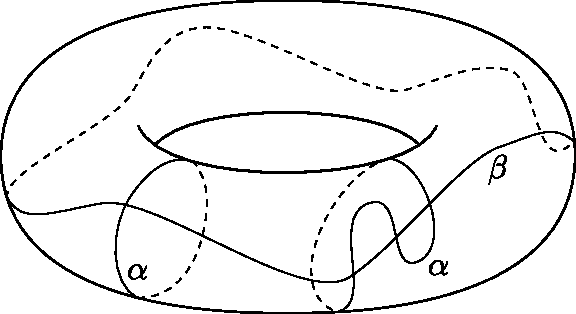
\includegraphics[width=2in]{905/Figures/30-torus-cycle-intersections.pdf}
\end{center}

\end{example}

This example exhibits a particularly interesting fragment of the statement
of Poincar\'e duality: In an even dimensional manifold -- say $n=2k$ -- the
cup product pairing gives us a nondegenerate symmetric bilinear form on 
$H^k(M)$. As indicated above, this can equally well be considered a bilinear
form on $H_k(M)$, and it is then to be thought of as describing the number of
points (mod 2) two $k$-cycles intersect in, when put in general position 
relative to one another. It's called the {\em intersection form}. We'll 
denote it by 
\[
\alpha\cdot\beta=\langle a\cup b,[M]\rangle\,,
\]
where again $a$ and $\alpha$ are Poincar\'e dual, and $b$ and $\beta$ are dual.

\begin{example} In terms of the basis $\alpha,\beta$, the intersection form
for $T^2$ has matrix 
\[
\left[\begin{array}{cc}0&1\\1&0\end{array}\right].
\]
This is a ``hyperbolic form.'' 
\end{example}

Let's discuss finite dimensional 
nondegenerate symmetric bilinear forms over $\FF_2$ in general.
A form on $V$ restricts to a form on any subspace $W\subseteq V$, but the 
restricted form may be degenerate. Any subspace has an 
{\em orthogonal complement} 
\[
W^\perp=\{v\in V:v\cdot w=0\,\,\hbox{for all}\,\,w\in W\} \,.
\]
\begin{lemma} The restriction of a nondegenerate bilinear form on $V$ to
a subspace $W$ is nondegenerate exactly when $W\cap W^\perp=0$. In that
case $W^\perp$ is also nondegenerate, and the splitting
\[
V\cong W\oplus W^\perp
\]
respects the forms. 
\end{lemma}
Using this easy lemma, we may inductively decompose a general (finite 
dimensional) symmetric bilinear form. First, if there is a vector $v\in V$
such that $v\cdot v=1$, then it generates a nondegenerate subspace and 
\[
V=\langle v\rangle\oplus\langle v\rangle^\perp\,.
\]
Continuing to split off one-dimensional subspaces brings us to the situation
of a nondegenerate symmetric bilinear form such that $v\cdot v=0$ for every
vector. Unless $V=0$ we can pick a nonzero vector $v$. Since the form is
nondegenerate, we may find another vector $w$ such that $v\cdot w=1$. The
two together generate a 2-dimensional hyperbolic subspace. Split it off 
and continue. We conclude:
\begin{prop} Any finite dimensional nondegenerate symmetric bilinear form
over $\FF_2$ 
splits as an orthogonal direct sum of forms with matrices $[1]$ and 
$\left[\begin{array}{cc}0&1\\1&0\end{array}\right]$.
\end{prop}

Let $\mathbf{Bil}$ be the set of isomorphism classes of finite dimensional 
nondegenerate symmetric bilinear forms over $\FF_2$. We've just given a classification of these things. This is a commutative monoid under orthogonal
direct sum. It can be
regarded as the set of nonsingular symmetric matrices modulo the equivalence
relation of ``similarity'': Two matrices $M$ and $N$ are {\em similar} if  
$N=AMA^T$ for some nonsingular $A$.
\begin{claim}
\begin{equation*}
\left[\begin{array}{ccc}
 & 1 & \\
1 & & \\
 & & 1
\end{array}\right]
\sim
\left[\begin{array}{ccc}
1 & & \\
& 1 & \\
& & 1
\end{array}\right]
\end{equation*}
\end{claim}
\begin{proof}
This is the same thing as saying that 
$\left[\begin{array}{ccc} & 1 & \\ 1 & & \\ & & 1\end{array}\right]=AA^T$ 
for some nonsingular $A$. Let 
$
A=\left[\begin{array}{ccc}1&1&1 \\ 1&0&1 \\ 0&1&1 \end{array}\right]$.
\end{proof}
It's easy to see that there are no further relations; 
$\mathbf{Bil}$ is the commutative monoid with two generators $I$ and $H$, 
subject to the relation $I+H=3I$. 

Let's go back to topology. Let $n=2$. Then you get an intersection pairing on $ H_1(M)$. Consider $\RP^2$. We know that $ H_1(\RP^2)=\FF_2$. This must be the form we labelled $I$. This says that anytime you have a nontrivial cycle on a projective plane, there's nothing you can do to remove its self interesections. You can see this. The projective plane is a M\"obius band with a 
disk sown on along the boundary. The waist of the M\"obius band serves as a
generating cycle. The observation is that if this cycle is moved to intersect 
itself tranversely, it must intersect itself an odd number of times. 

We can produce new surfaces from old by a process of ``addition.''
Given two connected surfaces $\Sigma_1$ and $\Sigma_2$, 
cut a disk out of each one and
sew them together along the resulting circles. This is the 
{\em connected sum} $\Sigma_1\#\Sigma_2$. 
\begin{prop} 
There is an isomorphism 
\[
H^1(\Sigma_1\#\Sigma_2)\cong H^1(\Sigma_1)\oplus H^1(\Sigma_2)
\]
compatible with the intersection forms. 
\end{prop}
\begin{proof}
Let's compute the cohomology of $\Sigma_1\#\Sigma_2$ using Mayer-Vietoris. 
The two dimensional cohomology of $\Sigma_i-D^2$ vanishes because the 
punctured surface retracts onto its 1-skeleton. The relevant fragment is
\[
0\to H^1(\Sigma_1\#\Sigma_2)\to H^1(\Sigma_1-D^2)\oplus H^1(\Sigma_2-D^2)\to
H^1(S^1)\xrightarrow{\delta} H^2(\Sigma_1\#\Sigma_2)\to0\,.
\]
The boundary map must be an isomorphism, because the connected sum is a
compact connected surface so has nontrivial $H^2$. We leave the verification
that the direct sum is orthogonal to you.
\end{proof} 
Write $\mathbf{Surf}$ for the set of homeomorphism classes of compact connected surfaces. Connected sum provides it with the structure of a commutative monoid. The classification of surfaces may now be summarized as folows:
\begin{theorem}
Formation of the intersection bilinear form gives an isomorphism of 
commutative monoids $\mathbf{Surf}\to\mathbf{Bil}$.
\end{theorem}
This is a kind of model result of algebraic topology! -- a complete
algebraic classification of a class of geometric objects. The oriented
surfaces correspond to the bilinear forms of type $gH$; $g$ is the
{\em genus}. But it's a little
strange. We must have a relation corresponding to $H\oplus I=3I$, namely
\[
T^2\#\RP^2\cong(\RP^2)^{\# 3}\,.
\]
You should verify this for yourself!
%The two-fold connected sum $\RP^2\#\RP^2$ is the Klein bottle $K$.  
%In fact, more generally
%\begin{claim}
%If $\Sigma$ is a nonoriented surface then $\Sigma\# T^2\cong\Sigma\# K$.
%\end{claim}

There's more to be said about this. Away from characteristic 2, symmetric
bilinear forms
and quadratic forms are interchangeable. But over $\FF_2$ you can ask for
a quadratic form $q$ such that 
\[
q(x+y)=q(x)+q(y)+x\cdot y\,.
\]
This is a ``quadratic refinement'' of the symmetric bilinear form.
Of course it implies that $x\cdot x=0$ for all $x$, so this will
correspond to some further structure on an oriented surface. This 
structure is a ``framing,'' a trivialization of the normal bundle of
an embedding into a high dimensional Euclidean space. There are then
further invariants of this framing; this is the story of the Kervaire
invariant.

